\section{机械能}\label{sec:8-7}

从斜面滚下的钢球撞在纸盒上(图 \ref{fig:8-10}),能将纸盒推动一段距离,表明滚动的钢球能够做功。
打桩机的重锤被举高以后,当它再落下时,能将木桩打入地里,表明这个重锤能够做功。
被压缩的弹簧(图 \ref{fig:8-11})一旦放松,能将它上面的砝码顶起,表明被压缩的弹簧能够做功。

\begin{figure}[htbp]
    \centering
    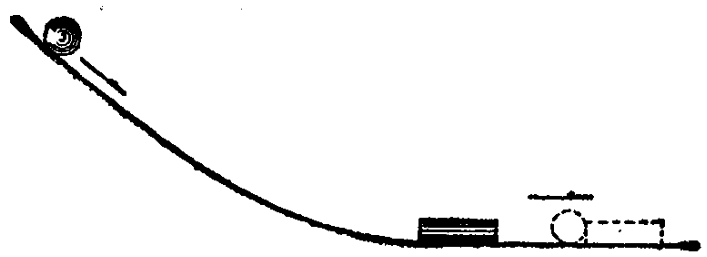
\includegraphics[width=0.6\textwidth]{../pic/czwl1-ch8-10}
    \caption{}\label{fig:8-10}
\end{figure}

\begin{figure}[htbp]
    \centering
    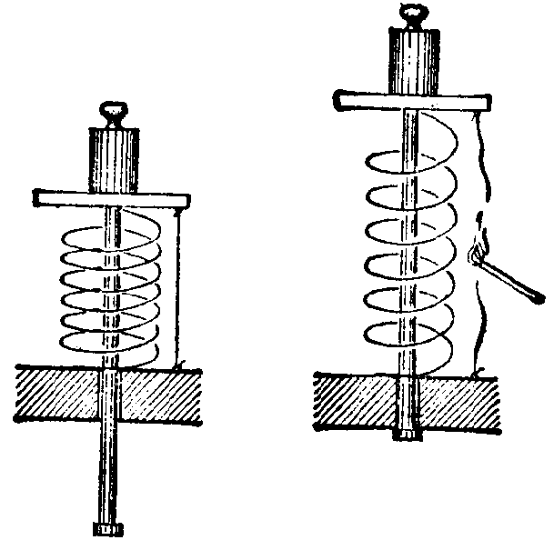
\includegraphics[width=0.4\textwidth]{../pic/czwl1-ch8-11}
    \caption{}\label{fig:8-11}
\end{figure}

一个物体能够做功,我们就说这个物体具有能。上面实验里的钢球、重锤、弹簧都具有能。
物体能够做的功越多,它具有的能就越多。



(1) 动能

滚动的钢球有能,是因为它在运动。\textbf{物体由于运动具有的能叫做动能}。
一切运动的物体都有动能。

在图 \ref{fig:8-10} 所示的实验中,让钢球从不同的高处滚下,可以看出,钢球原来的位置越高,
它滚下斜面后的速度越大,把纸盒推得就越远,做的功也就越多。
这表明运动物体的速度越大,它的动能就越多。
再让质量不同的钢球从同一高度滚下,可以看出质量较大的钢球把纸盒推得较远,做的功较多。
这表明运动物体的质量越大,它的动能就越多。

所以,\CJKunderwave{运动物体的速度越大,质量越大,它的动能就越多}。



(2) 势能

放在地上的重锤不能做功,只有把它举到高处,当它从高处落下来时才能做功。
重锤是由于被举到高处才具有能的。
自由状态的弹簧不能做功,只有把它压缩(或拉伸),当它被放松时才能做功。
弹簧是由于发生了弹性形变\footnotemark 才具有能的。
\footnotetext{外力撤消后,能完全恢复原来形状的形变叫做弹性形变。}

\textbf{物体由于被举高或者发生弹性形变而具有的能叫做势能}。
\CJKunderwave{物体被举得越高,质量越大,它的势能就越多。
弹性物体的弹性形变越大,它的势能就越多}。

物体的势能只有当物体的高度发生改变或者弹性形变的大小发生改变的时候才表现出来。
打桩机的重锤,只有当它落下的时候才做功——将木桩打入地里。
拉开了的弓,只有在手松开的时候才做功——将箭射出去。

物体通常既有动能又有势能。
例如飞行中的飞机,因为它在运动而具有动能,又因为它在高处,还具势能。

\begin{wrapfigure}[12]{r}{5cm}
    \centering
    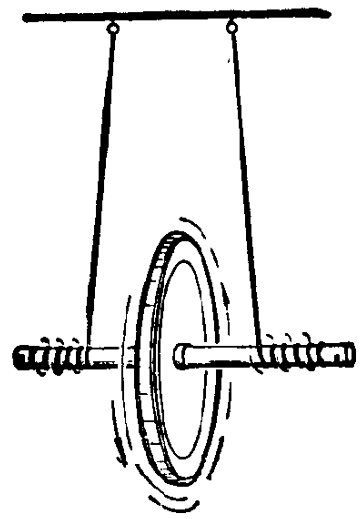
\includegraphics[width=4cm]{../pic/czwl1-ch8-12}
    \caption{}\label{fig:8-12}
\end{wrapfigure}

\textbf{有动能和势能统称为机械能}。



(3) 动能和势能的相互转化

物体具有的动能和势能可以相互转化。这种现象可以用滚摆(图 \ref{fig:8-12})来观察。
用手捻动滚摆的轴,使悬线缠在轴上,滚摆就上升。
滚摆升到顶点的时候,具有一定的势能。
这时松开手,滚摆就旋转着下降,势能随着它的下降而逐渐减少,
可是它越转越快,表示动能在逐渐增加,可见势能在转化为动能。
当悬线完全伸开,滚摆不再下降的时候,由于滚摆的继续旋转,它又开始绕着线上升。
在上升的过程中,动能逐渐减少,势能逐渐增加,动能又转化为势能。
上升到跟上一回差不多的高度,然后再下降,再上升。
这样,动能和势能不断地相互转化。
假如没有阻力,滚摆每次上升的高度都相同,
即在势能和动能的相互转化过程中滚摆的能的总量保持不变。


动能和势能相互转化的例子,在日常生活里也经常可以看到。
比如,托在手上的乒乓球有势能,当它离开手落向地板时,势能转化为动能,
当它撞击地板时发生弹性形变,动能转化为势能,
在它恢复原状的过程中,势能又转化为动能,使它离开地面向上弹起。
假如没有阻力,乒乓球可以弹起到原来的高度,即它的能的总量保持不变。

从上面讲的和其他许多现象的研究中,可以得到下面的结论:

\textbf{势能可以转化为动能,动能可以转化为势能}。

\textbf{在势能和动能的相互转化过程中,机械能的总量保持不变}。

实际上,由于存在摩擦阻力和空气阻力,滚摆每次上升的高度都逐渐减小,乒乓球每次弹起的高度也都比前一次低。
滚摆和乒乓球失去的机械能并没有消灭,而是转化成另一种形式的能——热能。
关于机械能和热能相互转化的知识,我们将在初三物理中学习。



\lianxi

(1) 除了课本中已经讲过的,再举三个物体有势能的例子。

(2) 除了课本中已经讲过的,再举三个物体有动能的例子。

(3) 自行车下坡,不踩脚踏板,速度也越来越快,为什么?

(4) 你骑自行车时,在上坡前往往要加紧蹬几下;汽车司机在开车上坡前,也往往要加大油门。
从能的转化来说明这样做的好处。

(5) 怎样向地板上抛乒乓球,才能使它弹跳到高于抛球处的位置?
根据动能、势能的相互转化规律来说明那样抛的理由。

